% ---
% Arquivo com a execução do Trabalho de Conclusão de Curso dos alunos
% Gabriel Takaoka Nishimura, Felippe Demarqui Ramos e Vivian Kimie Isuyama 
% da Escola Politécnica da Universidade de São Paulo
% ---
	\chapter{Execução}\label{cap-execucao}
	
	\section{Arquitetura}
	
	\subsection{Codificador}
	
	Conforme apontado no capítulo de Metodologia, a arquitetura do codificador Reed Solomon foi construída para um código (15, 7), portanto contando com 8 registradores em série. Os multiplicadores foram feitos com uma tabela,  que recebe duas entradas e retorna uma saída, de maneira a simplificar o trabalho de fazer uma função utilizando lógica combinatória. Já os somadores são equivalentes à função de OU exclusivo, ou XOR, com duas entradas e uma saída de 4 bits cada - ou seja, um símbolo. Além destes, os módulos básicos ainda compreendem um multiplexador, que seleciona um entre dois símbolos.
	
	Diagrama do codificador
	
	O comportamento de codificação de uma mensagem pode ser exemplificado pela seguinte simulação, onde se observa a entrada de uma mensagem de 7 símbolos e a saída de um bloco de 15 símbolos, sendo 8 de paridade.	
	
	
	\subsection{Decodificador}
	
	A arquitetura do decodificador segue o diagrama funcional da figura X do capítulo de Metologia. Desta forma, o desenvolvimento pode ser separado em quatro partes principais, apresentadas a seguir.
	
	Cálculo das Síndromes
	
	O cálculo das síndromes é feito de forma iterativa, durando tantos ciclos quanto forem os símbolos da mensagem. O cálculo de cada síndrome é independente dos cálculos das demais, e depende apenas dos símbolos de entrada e de cada uma das raízes do polinômio codificador, de alpha0 a alpha7 neste caso.
	
	*diagrama de cálculo das síndromes*
	
	A simulação a seguir representa o caso em que existem erros na mensagem codificada, o que é indicado por síndromes diferentes de 0000.
	
	*simulação das síndromes*
	
	Módulo de Berlekamp-Massey
	
	O módulo de Berlekamp-Massey foi implementado de forma a primeiramente calcular as localizações dos erros, ou seja, os coeficientes do polinômio localizador de erros, representados por Lamba, e guardados em registradores, para o posterior cálculo dos valores dos erros. Os valores de erros são calculados então, com as síndromes e localizações de erro.
	
	Diagrama do módulo
	
	Simulação
	
	% ---
	\section{Hardware}
	% ---
	\subsection{Transmissor}
	\subsubsection{Conversor Digital-Analógico}
		 Os requisitos para o transistor de potência realizando transmissão via luz são:

		\begin{itemize}
			\item Tensão de base/gate compatível com 3.3V;
			\item Corrente de saída compatível com LED de alta potência, no mínimo 750mA;
			\item Resposta de base/gate a $V_{on(FPGA)}$ de no máximo 1us;
		\end{itemize}
		
		Alguns dos parâmetros são decisões de projeto, como a utilização de níveis TTL para chaveamento do transistor (3.3V ou 5V), e também requisitos da norma IEEE, como frequência de operação a 200kHz (nesse caso deseja-se um transistor com $T_{rise}$ e $T_{fall}$ de no mínimo 10-100 vezes menor que o período da onda transmitida - no caso $5\mu$$s/100 = 50ns$).
		O componente escolhido foi um MOSFET de Potência, mais especificamente o IRLZ14, pois é um transistor de nível lógico, então tem o GATE compatível com voltagens de microcontrolador. 
		
		\begin{figure}[htb]
			\caption{\label{fig_transfer_carac_irlz14} Características de transferência do MOSFET de potência IRLZ14.}
			\centering		%  trim={<left> <lower> <right> <upper>} 
			\includegraphics[page=3, width=0.7\textwidth, trim={12cm 16.5cm 2.2cm 5cm}, clip]{circuits/irlz14.pdf}
			\legend{Fonte: Vishay Siliconix.}
		\end{figure}
	
		De acordo com função de transferência da \autoref{fig_transfer_carac_irlz14}, a VGS=3.3V ele permite corrente de dreno de 2A. A datasheet também especifica parâmetros de resposta dinâmica do circuito, como seu $T_{rise}$, $T_{fall}$, que estão disponibilizados na tabela abaixo.
		
		\begin{table}[ht]
			\caption{Características Dinâmicas do MOSFET IRLZ14}
			\centering
			\begin{tabular}{c c}
				\hline
				Parâmetro  & Valor  \\ \hline
				$T_{rise}$ & 110 ns \\
				$T_{fall}$ & 26 ns  \\ \hline
			\end{tabular}
			\label{tab_irlz14_timing}
			\legend{Fonte: Vishay Siliconix.}
		\end{table}
	
		O circuito proposto é 

	\subsubsection{Transmissão de Luz}
		
		Para realizar a transmissão de luz a distâncias de pelo menos um metro, será necessária a utilização de um LED de potência. O LED deverá atender a requisitos de altas frequência e resposta luminosa de acordo com seu chaveamento.
		
%		\begin{figure}[htb]
%			\caption{\label{fig_pulse_handling_led} Gráfico da capacidade de manuseio de pulso do LED LUW-W5AM. D: Duty Cycle, Ts = 25 C}
%			\centering									%  trim={<left> <lower> <right> <upper>} 
%			\includegraphics[page=15, width=0.5\textwidth, trim={2.5cm 4.6cm 11.5cm 15.6cm}, clip]{circuits/led_luw_w5am.pdf}
%			\legend{Fonte: OSRAM LUW W5AM Datasheet.}
%		\end{figure}

		 a frequências altas com alta corrente são necessários cuidados especiais para projetar um circuito que oscila corretamente de acordo com o sistema de chaveamento anterior.
		
	\subsection{Receptor}
	\subsubsection{Recepção Luminosa}
		
		A photodiode is a semiconductor device that converts light into current. The current is generated when photons are absorbed in the photodiode. A small amount of current is also produced when no light is present. Photodiodes may contain optical filters, built-in lenses, and may have large or small surface areas. Photodiodes usually have a slower response time as their surface area increases. The common, traditional solar cell used to generate electric solar power is a large area photodiode.
		
		Photodiodes are similar to regular semiconductor diodes except that they may be either exposed (to detect vacuum UV or X-rays) or packaged with a window or optical fiber connection to allow light to reach the sensitive part of the device. Many diodes designed for use specifically as a photodiode use a PIN junction rather than a p–n junction, to increase the speed of response. A photodiode is designed to operate in reverse bias.[1]

%		https://www.aptechnologies.co.uk/images/img/ODC/PV_and_PC_Modes.png
		
		
	\subsubsection{Amplificador de Transimpedância}
	
	\subsubsection{Conversor Analógico-Digital}
	
	\section{Software}
		Com os dados codificados, enviados via luz, recebidos via luz e decodificados, é possível realizar 